\documentclass{article}
\usepackage{setspace}
\usepackage{arabtex}
\usepackage{utf8} 
\usepackage{hyperref} 
\usepackage{graphicx}
\usepackage{subcaption}
\usepackage{tabularx}
\usepackage{geometry}
\usepackage{lipsum}
\usepackage{listings}
\usepackage{color}
\usepackage{enumitem}

\definecolor{dkgreen}{rgb}{0,0.6,0}
\definecolor{gray}{rgb}{0.5,0.5,0.5}
\definecolor{mauve}{rgb}{0.58,0,0.82}

\newcounter{magicrownumbers}
\newcommand\rownumber{\stepcounter{magicrownumbers}\arabic{magicrownumbers}}

\lstset{frame=tb,
	language=Java,
	aboveskip=3mm,
	belowskip=3mm,
	showstringspaces=false,
	columns=flexible,
	basicstyle={\small\ttfamily},
	numbers=none,
	numberstyle=\tiny\color{gray},
	keywordstyle=\color{blue},
	commentstyle=\color{dkgreen},
	stringstyle=\color{mauve},
	breaklines=true,
	breakatwhitespace=true,
	tabsize=3
}

\setcounter{tocdepth}{2}
\hypersetup{
	colorlinks,
	citecolor=[rgb]{0,0.5,0.5},
	filecolor=[rgb]{0,0.5,0.5},
	linkcolor=[rgb]{0,0.5,0.5},
	urlcolor=[rgb]{0,0.5,0.5}
}

\date{}
\title{
	Bank Automated Teller Machines \\
	\large Software Engineering (CS385T) Project }

\author{
	\setcode{utf8}
	\RL{ريم علي الغامدي} 
	\\\texttt{437004875}
	\\[3ex]
	\RL{سارة خالد آل حسين} 
	\\\texttt{436006939}
	\\[3ex]
	\RL{عبير عزت} 
	\\\texttt{436200058}
	\\[3ex]
	\RL{لمياء القحطاني} 
	\\\texttt{437004164}
}

\begin{document}
	
	
	\pagenumbering{gobble}
	\maketitle
	\newpage
	\addcontentsline{toc}{section}{Member Roles}
	
	\def\arraystretch{2}
	\begin{table}[h!]
		\begin{center}
			\caption{Member Roles}
			\begin{tabularx}{\textwidth}{r|c|X}
				\textbf{Name} & 
				\textbf{ID} & 
				\textbf{Responsibility}\\
				\hline
				\RL{ريم علي الغامدي} &
				\texttt{437004875} &
				Transfer
				\\
				\hline
				\RL{سارة خالد آل حسين} &
				\texttt{436006939} &
				Withdraw
				\\
			\hline
				\RL{شهد} &
				\texttt{436006939} &
				validate
				\\
				\hline
				\RL{عبير عزت} &
				\texttt{436200058} &
				Deposit
				\\
			\hline
				\RL{لمياء القحطاني} &
				\texttt{437004164} &
				Retrieve
				\\
				
			\end{tabularx}
		\end{center}
	\end{table}

	\newpage
	\pagenumbering{arabic}
	\addcontentsline{toc}{section}{Table of Contents}\tableofcontents
	\newpage	
	\doublespacing
	\newpage
	
	

	\section{Introduction}
	\subsection{Purpose}
	\subsection{Scope}
	\subsection{Generic Software Model}
	\section{Requirement Specifications}
	\subsection{Functional Requirements}


	\begin{enumerate}[label*=\arabic*.]
		\item The ATM shall validate the user.
		\item The user shall be able to retrieve account information.	
		\item The user shall be able to withdraw money.
		\item The user shall be able to deposit money.
		\item The user shall be able to transfer money to another account.
	\end{enumerate}

	\subsection{Non-functional Requirements}
	\begin{enumerate}
		\item The system must be secure.
		\item The system must be available 24H.
	\end{enumerate}

	\newpage\subsection{Functional Requirements Description}
	\setcounter{magicrownumbers}{0}
	\def\arraystretch{2}
	\begin{table}[h!]
		\begin{center}
			\begin{tabularx}{\textwidth}{r|X|X}
				\textbf{ID} & 
				\textbf{Requirement} & 
				\textbf{Description}\\
				\hline
				\rownumber &
				The ATM shall validate the user. &
				ATM should ask for the user card and PIN code, then send these information to the bank to validate the user, if PIN is correct bank sends the user account to the ATM
				\\
				\hline

				\rownumber &
				The user shall be able to retrieve account information. &
				After the user is validated, the user should be able to get account information. Including current balance, debt, number of cards activated, and the last transactions.
				\\
				\hline
				\rownumber &
				The user shall be able to withdraw money. &
				After the user is validated, the user should be able to get withdraw money from account if withdrawn amount is less than the balance.
				\\
				\hline
				\rownumber &
				The user shall be able to deposit money. &
				After the user is validated, the user should be able to deposit money into account if money is validated to be real and undamaged.
				\\
				\hline
				\rownumber &
				The user shall be able to transfer money to another account. &
				After the user is validated, the user should be able to transfer money from account to any other account as long as IBAN entered is correct and amount transferred is less than the balance.
				\\	
			\end{tabularx}
		\end{center}
	\end{table}

	\newpage\subsection{Non-functional Requirements Description}
	\setcounter{magicrownumbers}{0}
	\def\arraystretch{2}
	\begin{table}[h!]
		\begin{center}
			\begin{tabularx}{\textwidth}{r|X|X}
				\textbf{ID} & 
				\textbf{Requirement} & 
				\textbf{Description}\\
				\hline
				\rownumber &
				The system must be secure. &
				The system must be impossible to hack, connection must be secure and data must be encrypted and layered.
				\\
				\hline

				\rownumber &
				The system must be available 24H. &
				The system must never fail or else the user or the bank might lose money.
				\\
			
			\end{tabularx}
		\end{center}
	\end{table}

	\section{Design}
	\newpage\subsection{Validate User}
	\newpage\subsection{Retrieve Account Information}
	\newpage\subsection{Withdraw Money}
	\newpage\subsection{Deposit Money}
	\newpage\subsection{Transfer}
		\subsubsection{Use Case Scenario}
		\textbf{Use Case Name:}	transfer money to another account.
		\newline\textbf{Goal:} to transfer money.
		\newline\textbf{Actors:} user, receiver, ATM, Bank 	
		\newline\textbf{Precondition:} user is validated 	
		\newline\textbf{Primary Scenario:}	
			\begin{enumerate}[label*=\arabic*.]
				\item ATM shows menu.
				\item user chooses "transfer money".
				\item ATM asks user to enter receiver's IBAN.
				\item If IBAN is correct, ATM asks for the amount transferred.
				\item If the amount is available in the user's account, money is transferred to receiver's account.
				\item User quits.
				\item ATM ejects the card.
			\end{enumerate}
		\textbf{Variant:}\newline	
			\hspace*{5mm}4a. If IBAN is incorrect, banks asks the user to enter it again.\newline
			\hspace*{5mm}5a. If the amount transferred is less than the user's current balance, the ATM shows an error message.\newline
			\hspace*{5mm}*. The user may cancel the session; the ATM ejects the card.

		\newpage\subsubsection{Use Case Diagram}
		\begin{figure}[h!]
		  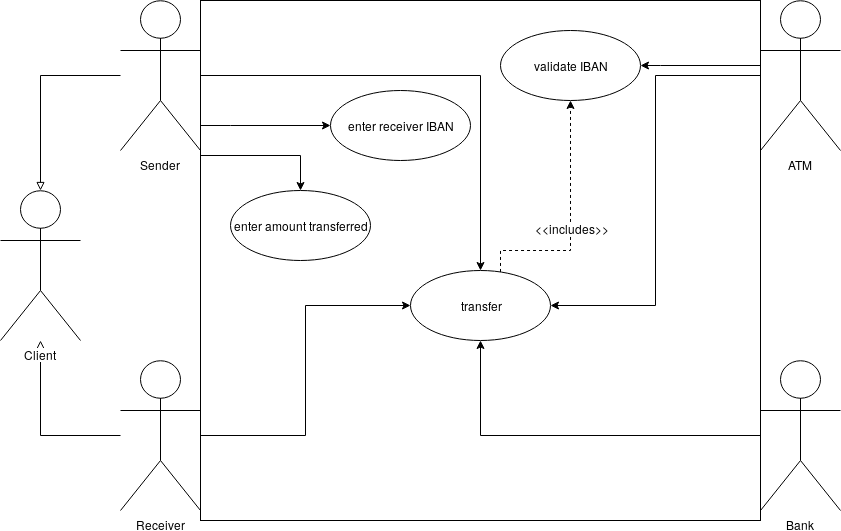
\includegraphics[width=\linewidth]{img/transfer_usecase.png}
		\end{figure}

		\newpage\subsubsection{Sequence Diagrams}
		\begin{figure}[h!]
		  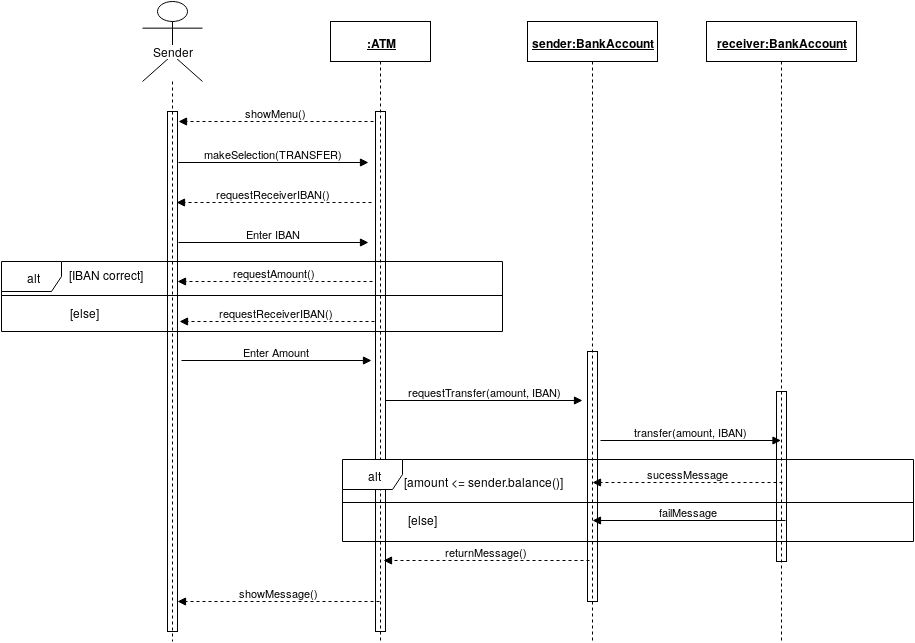
\includegraphics[width=\linewidth]{img/transfer_sequence.png}
		\end{figure}

		\newpage\subsubsection{Collaboration Diagram}	
		\begin{figure}[h!]
		  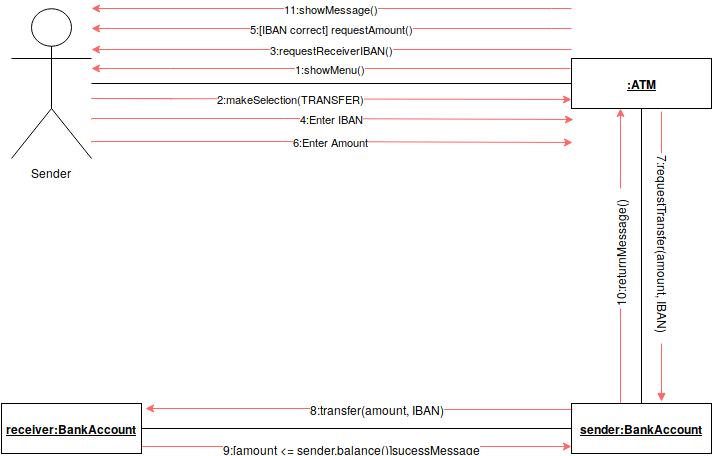
\includegraphics[width=\linewidth]{img/transfer_collaboration.png}
		\end{figure}

		\newpage\subsubsection{Activity Diagram}
		\begin{figure}[h!]
			\begin{center}
				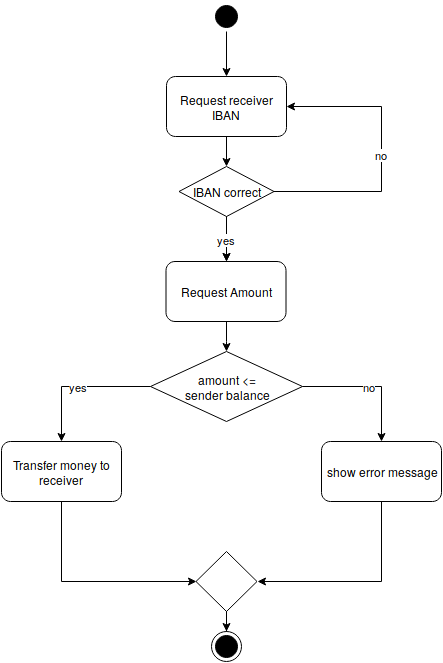
\includegraphics[height=\linewidth]{img/transfer_activity.png}
			\end{center}
		\end{figure}

		\newpage\subsubsection{Flow Chart}

	\newpage\subsection{For The Whole System}
	\subsubsection{Context Diagram}	
	\subsubsection{Use-case Diagram}
	\subsubsection{Component diagram}
	\subsubsection{Deployment diagram}
	\subsubsection{Data flow Diagram}		
	\subsubsection{Class Diagram}
	\subsubsection{Object Diagram}		
	\subsubsection{State Chart Diagram}
	\subsubsection{Architectural patterns}


	\newpage
	\addcontentsline{toc}{section}{References}
	\bibliographystyle{ieeetr}
	\bibliography{References}

\end{document}
